\documentclass[slovak, 12pt, Times New Roman]{article}
\usepackage[slovak]{babel}
\usepackage[utf8]{inputenc} 
\usepackage[top=1in, bottom=1in, left=1in, right=1in]{geometry}
\usepackage{graphicx}
\usepackage{hyperref}
\hypersetup{
    colorlinks=true, %set true if you want colored links
    linktoc=all,     %set to all if you want both sections and subsections linked
    linkcolor=black,  %choose some color if you want links to stand out
}
\usepackage{fancyhdr}

--INSERT INTO VAZNI VALUES(1,'Ferko','Mrkvcicka',1,default,'12/10/2022',default,3,1);
--INSERT INTO DOZORCOVA VALUES(1,'Rastislav','Dolina',1,1,950);
--INSERT INTO POSTY VALUES(1,1,'poslal');
--INSERT INTO BLOKY VALUES(1,'lave kridlo',122,244,default,3);
--INSERT INTO CELY VALUES(1,2,default);
--INSERT INTO HODNOSTI VALUES('1','Plukovnik',1);
--INSERT INTO PLATOVE_SKUPINY VALUES(1,600,990);
--INSERT INTO PRACE VALUES(1,'pradelna',100);
--INSERT INTO SLUZBY VALUES(1,1,1,default);
--INSERT INTO TYPY_SLUZIEB VALUES(1,'ranna',6,14.5);
--INSERT INTO PRIESTUPKY VALUES(1,1,default,'bitka');
DELETE * FROM VAZNI;

\begin{document}
	\thispagestyle{fancy}
	\chead{Slovenská technická univerzita v Bratislave, Fakulta elektrotechniky a informatiky, Ilkovičova 3, 812 19 Bratislava}
	\topskip70mm
		\begin{center}\huge{Softvérová špecifikácia\\ WebRočenka\par}\end{center}
	\title{Softvérová špecifikácia WebRočenka}
	\date{}

	\begin{minipage}[b]{\textwidth}
	    \vspace{110mm}	 
	    \large   
	    V Bratislave \hspace{90mm} Vypracoval:\\
	    31 Októbra 2014 \hspace{81mm} Gabriel Kerekeš
	    \vspace{-20mm} 
	\end{minipage}
	\topskip0pt
	\clearpage
	\paragraph{Zaznamenavanie zmien}
	\clearpage
	\tableofcontents
	\clearpage
	\section{Používateľská špecifikácia}
		\subsection{Úvod do problematiky}
			WebRočenka je softvér, ktorý bude umožnovať komunikáciu medzi absolventami stredných a vysokých škôl, tak, že bude vedieť evidovať školy, odbory, triedy, študentov a učiteľov. Študenti a učitelia sa budú registrovať sami a po registrácií sa môžu pokúsiť prihlásiť do triedy/odboru/krúžku, ďalej len ako trieda, (musia splniť podmienky dané správcom triedy). Neregistrovaní a neprihlásení používatelia budú môcť vyhľadať triedu, avšak neuvidia žiadne podrobnejšie informácie o nej. Takisto nebudú môcť prezerať profily iných používateľov. Každý užívateľ bude mať možnosť uchovávať, aktualizovať a meniť údaje o sebe (kontaktné údaje, všeobecné informácie, fotku, ...). Školy, ktoré budú chýbať v evidencii, budú registrované správcom softvéru na základe požiadavky od študentov/učiteľov. Triedy budú zakladané študentami, ktorí by sa tiež mali najprv uistiť, že daná trieda ešte neexistuje, aby sa predišlo duplicitným záznamom. Študent, ktorý triedu vytvoril sa stáva správcom tejto triedy a má následujúce oprávnenia:
			\begin{itemize} \itemsep0pt \parskip0pt \parsep0pt
				\item pridať/odobrať uživateľa z triedy
				\item zvoliť spolusprávcu
				\item zadať podmienky podmieňujúce pridanie do triedy (kontrolná otázka, scvhálenie správcom triedy, ...)
			\end{itemize}
			Každa trieda bude mať spoločnú nástenku, na ktorú može každý používateľ pridávať príspevky. Takisto bude spoločná nástenka pre celú školu. Systém bude tiež umožňovať vytváranie spoločných eventov pre celú školu/triedu a tiež aj zvlášť pre študentov a učiteľov. Študenti budú mať možnosť komunikovať medzi sebou prostredníctvom súkromných správ, ktoré bude možné zablokovať, aby sa predišlo zbytočnému obťažovaniu. Správca triedy bude mať tiež možnosť posielať hromadné maily používateľom vo svojej triede, ak má používateľ túto funkciu povolenú.
		\subsection{Používateľské požiadavky}
			\subsubsection{Funkcionálne požiadavky}
				\begin{itemize} \itemsep0pt \parskip0pt \parsep0pt
					\item neregistrovaný/neprihlásený používateľ by mal vedieť vyhľadať triedu, nemal by byť schopný vidieť nástenky škôl/tried, nemal by vedieť posielať súkromné správy, ani prehliadať profily ostatných užívateľov
					\item používateľ sa má vedieť zaregistrovať/prihlásiť
					\item používateľ má vedieť vytvoriť novú triedu - stane sa jej správcom
					\item používateľ má vedieť upravovať svoje údaje
					\item používateľ má vedieť komunikovať (odosielať, prijímať) cez súkromné správy s ďalšími členmi triedy, keď to povolujú 			nastavenia oboch strán tak aj mimo triedy
					\item používateľ má vedieť prispievať na nástenku školy/triedy
					\item používateľ má vedieť požiadať o pridanie do triedy
					\item používateľ má vedieť triedu opustiť
					\item používateľ má vedieť vytvoriť udalosť triedy ak je pridaný do tejto triedy
					\item používateľ má vedieť požiadať správcu systému o pridanie školy do systému
					\item správca triedy má vedieť pridať/odobrať užívateľa
					\item správca triedy má vedieť upravovať údaje triedy
					\item správca triedy má vedieť upraviť vstupné podmienky pre prijatie do triedy
					\item správca triedy má vedieť zvoliť nového/ďalšieho správcu
					\item správca triedy má vedieť rozoslať e-mail/súkromnú správu všetkým užívateľom v triede
					\item správca systému má vedieť odstrániť triedu/školu/používateľa
				\end{itemize}
			\subsubsection{Nefunkcionálne požiadavky}
				\begin{itemize} \itemsep0pt \parskip0pt \parsep0pt
					\item aktualizácie možné za behu systému					
					\item intuitívne používateľské rozhranie
				\end{itemize}
			\subsubsection{Merateľné požiadavky}
				\begin{itemize} \itemsep0pt \parskip0pt \parsep0pt
					\item maximálny downtime systému 10 minút
					\item schopnosť evidovať až 5.5 milióna používateľov, 500-tisíc tried/odborov/škôl
				\end{itemize}
			\subsubsection{Doménové požiadavky}
				\begin{itemize} \itemsep0pt \parskip0pt \parsep0pt
					\item systém musí zabezpečovať ochranu záznamov a osobných údajov podľa paragrafu 7 zákona 428 / 2002
							Z.z.
				\end{itemize}
				\clearpage
	\section{Systémová špecifikácia}
		\subsection{Diagram prípadov použitia}
			\begin{figure}[!htb]
				\centering
				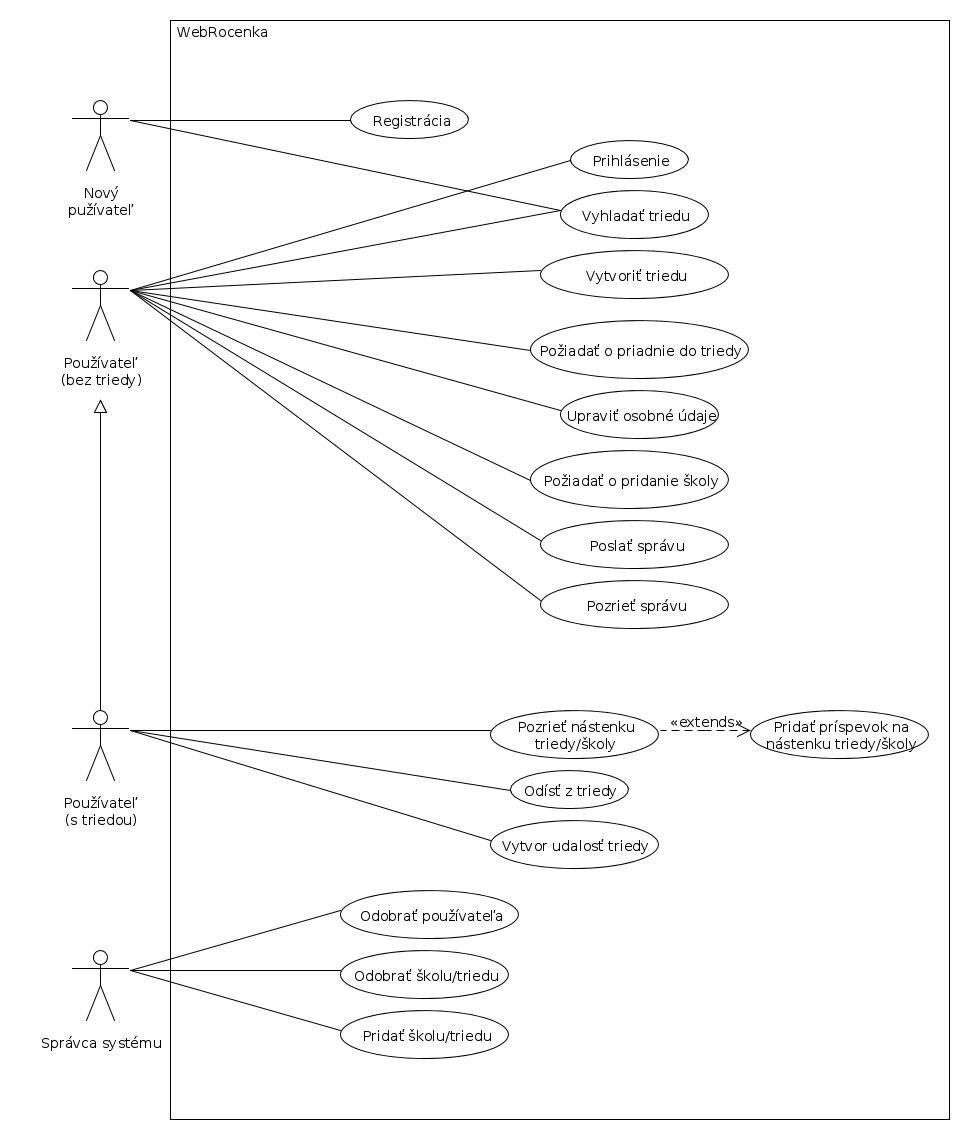
\includegraphics[scale=0.35]{useCaseBasic.jpg}
				\caption{Diagram prípadov použitia}
				\label{fig:Reinforcement}
			\end{figure}
		\clearpage
		\subsection{Role jednotlivých hráčov}
			\subsubsection{Neregistrovaný používateľ}
				Neregistrovaný používateľ sa môže registrovať a začať používať WebRočenku. Tiež má možnosť vyhľadať triedy/školy, čo je dôležité, aby zistil či sa mu oplatí registrovať. 
			\subsubsection{Prihlásený používateľ (bez triedy)}
				Prihlásený používateľ bez triedy môže vyhľadať triedu, požiadať o pridanie do triedy alebo môže vytvoriť vlastnú triedu. Môže požiadať o pridanie školy do systému. Môže vyhľadávať ľudí, posielať/prijímať súkromné správy. Môže upravovať svoje osobné údaje.
			\subsubsection{Prihlásený používateľ (s triedou)}
				Prihlásený používateľ s triedou si môže pozrieť nástenky tried/škôl, ktorých je členom. Na tieto nástenky môže zároveň aj pridávať príspevky. Triedu môže opustiť. Môže tiež vytvárať eventy pre celú triedu.
			\subsubsection{Správca systému}
				Správca systému je zodpovedný za pridávanie škôl do systému na základe požiadaviek od používateľov. Ďalej môže triedy/školy vymazávať zo systému (napr. pri vymyslených triedach, prázdnych školách, ...). Môže aj vymazať používateľov, ktorý sa napr. nevhodne správajú.
		\subsection{Tabuľky prípadov použitia}
			\begin{tabular} {|p{10mm}|p{40mm}|p{60mm}|p{40mm}|}
	  			\hline 
	  			\textbf{ID} & \textbf{Názov} & \textbf{Podmienka} & \textbf{Hráči} \\ 
	  			\hline
	  			1 & Pridať príspevok na nástenku triedy  & Používateľ musí byť prihlásený do príslušnej triedy & Používateľ s triedou \\
	  			\hline
	  			\multicolumn{4}{|c|} {\textbf{Postupnosť}} \\
	  			\hline
	  			\multicolumn{4}{|p{160mm}|} {1. Používateľ sa prihlási 2. Používateľ klikne na triedu v zozname svojích tried 3. Klikne na 'Zobraziť nástenku' 4. Klikne na 'Pridať príspevok' 5. Napíše príspevok 6. Klikne na 'Odoslať príspevok'}\\
	  			\hline
	  		\end{tabular}
	  		\\
	  		\vspace{2cm}
	  		\\
	  		\begin{tabular} {|p{10mm}|p{40mm}|p{60mm}|p{40mm}|}
	  			\hline 
	  			\textbf{ID} & \textbf{Názov} & \textbf{Podmienka} & \textbf{Hráči} \\ 
	  			\hline
	  			2 & Požiadať o pridanie školy & Používateľ musí byť prihlásený & Prihlásený používateľ \\
	  			\hline
	  			\multicolumn{4}{|c|} {\textbf{Postupnosť}} \\
	  			\hline
	  			\multicolumn{4}{|p{160mm}|} {1. Používateľ sa prihlási 2. Používateľ klikne na 'Support' tlačítko 3. Klikne na 'Odoslať žiadosť na pridanie školy' 4. Vyplní formulár 5. Klikne na 'Odoslať žiadosť'}\\
	  			\hline
	  		\end{tabular}
	  		\\
	  		\vspace{2cm}
	  		\\
	  		\begin{tabular} {|p{10mm}|p{40mm}|p{60mm}|p{40mm}|}
	  			\hline 
	  			\textbf{ID} & \textbf{Názov} & \textbf{Podmienka} & \textbf{Hráči} \\ 
	  			\hline
	  			3 & Pridať triedu & Existuje požiadavka na pridanie & Správca systému \\
	  			\hline
	  			\multicolumn{4}{|c|} {\textbf{Postupnosť}} \\
	  			\hline
	  			\multicolumn{4}{|p{160mm}|} {1. Správca sa prihlási 2. Klikne na 'Požiadavky na pridanie škôl' 3. Klikne na 'Zobraziť nové'' 4. Klikne na zvolenú žiadosť 5. Skontroluje správnosť formuláru 6. Zistí či daná škola existuje/existovala 7. Klikne na pridať školu 8. Systém automaticky podľa formuláru školu pridá}\\
	  			\hline
	  			\multicolumn{4}{|c|} {\textbf{Poznámky}} \\
	  			\hline
	  			\multicolumn{4}{|p{160mm}|} {Ak formulár nieje správne vyplnení, chyby, ktoré správca dokáže opraviť opraví, inak požiada používateľa o nové vyplnenie žiadosti. Ak škola neexistuje v skutočnosti tak ju samozrejme nepridá.}\\
	  			\hline
	  		\end{tabular}
	  	\clearpage
		\subsection{Diagramy aktivít a sekvenčné diagramy}
			\begin{figure}[!htb]
				\centering
				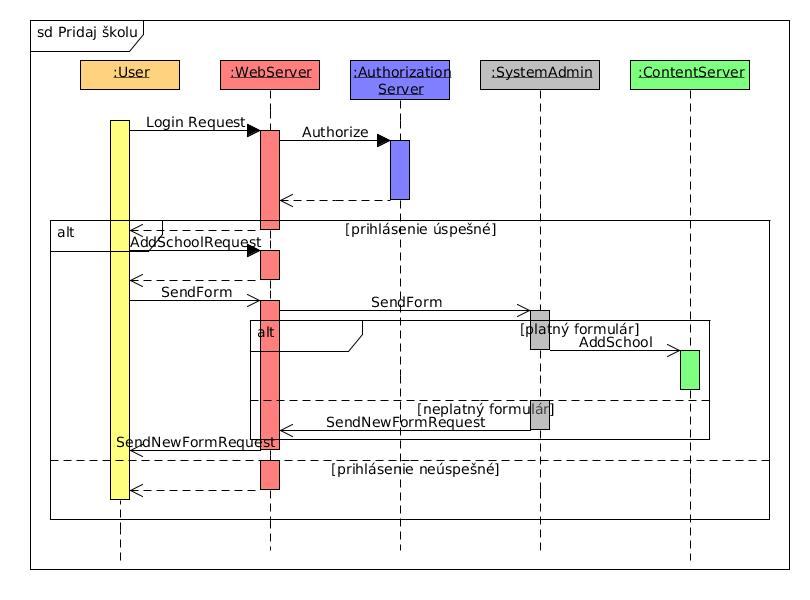
\includegraphics[width = 16cm, height = 15cm]{AddSchoolSequence.jpg}
				\caption{Sekvenčný diagram pridania školy do systému}
				\label{fig:Reinforcement}
			\end{figure}
		%\clearpage
			\begin{figure}[!htb]
				\centering
				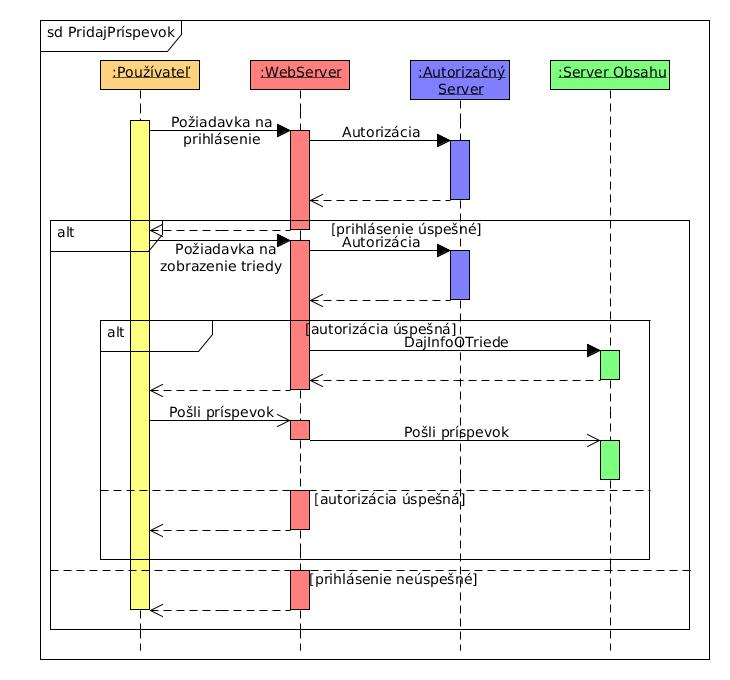
\includegraphics[width = 16cm, height = 15cm]{AddPostSequence.jpg}
				\caption{Sekvenčný diagram pridania príspevku na nástenku triedy}
				\label{fig:Reinforcement}
			\end{figure}
			\begin{figure}[!htb]
				\centering
				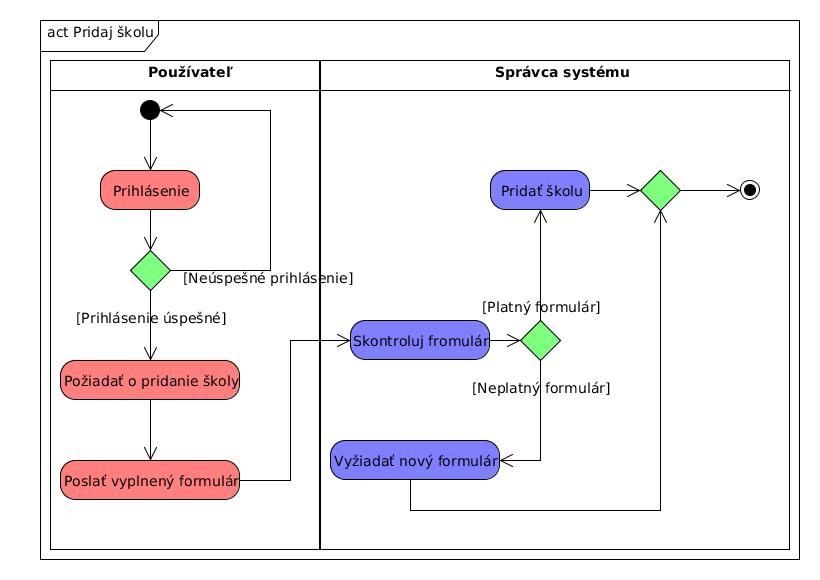
\includegraphics[width = 16cm, height = 9cm]{AddSchoolActivity.jpg}
				\caption{Aktivity diagram pridania školy do systému}
				\label{fig:Reinforcement}
			\end{figure}
			\begin{figure}[!htb]
				\centering
				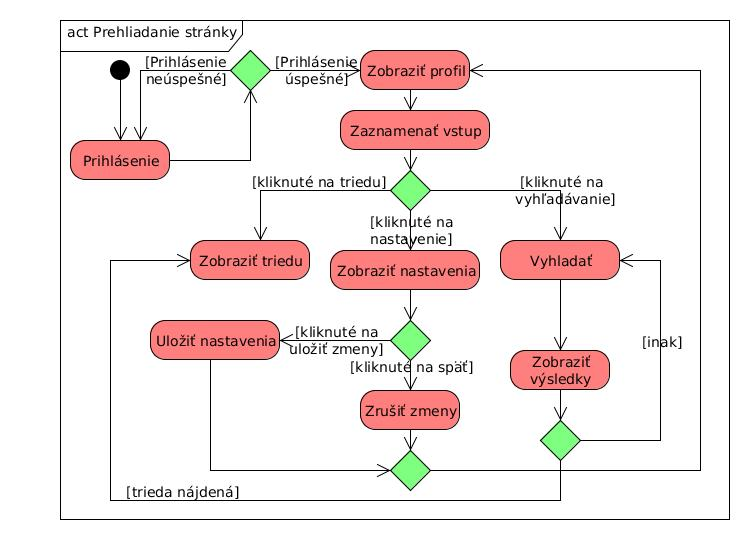
\includegraphics[width = 16cm, height = 9cm]{AddPostActivity.jpg}
				\caption{Aktivity diagram priehliadania stránky	}
				\label{fig:Reinforcement}
			\end{figure}
		\clearpage
		\subsection{Stavový diagram}
			\begin{figure}[!htb]
				\centering
				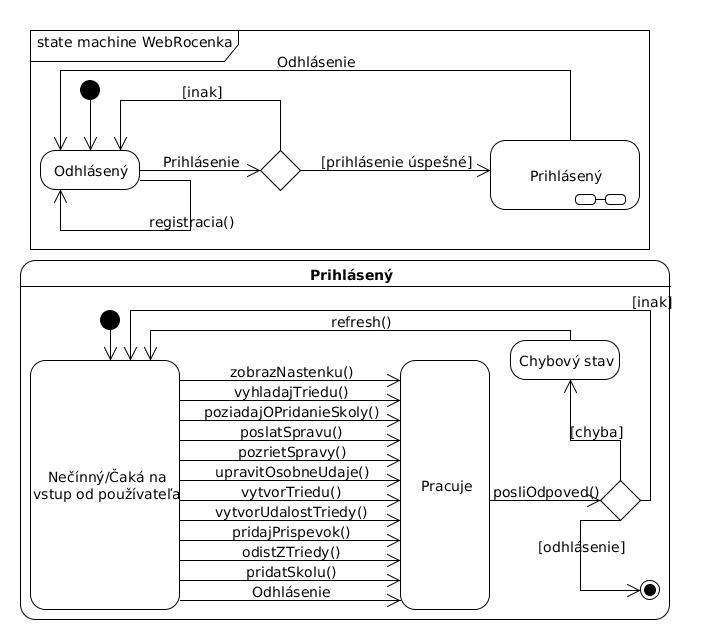
\includegraphics[width = 16cm, height = 17cm]{StateMachine.jpg}
				\caption{Stavový diagram systému}
				\label{fig:Reinforcement}
			\end{figure}
			%\vspace{2cm}
			\begin{tabular} {|p{4cm}|p{11cm}|}
				\hline
				\textbf{Stav} & \textbf{Popis} \\
				\hline
				Odhlásený & Používateľ je odhlásený a systém čaká na jeho prihlásenie/registráciu\\
				\hline
				Prihlásený & Používateľ je prihlásený a systém nečinný\\
				\hline
				Nečinný & Systém čaká na používateľov vstup\\
				\hline
				Pracuje & Systém spracováva používateľov vstup\\
				\hline
				Chybový stav & Systém sa nachádza v chybovom stave; používateľ zavolá refresh()\\
				\hline
			\end{tabular}

			\vspace{2cm}

			\begin{tabular} {|p{4.5cm}|p{10.5cm}|}
				\hline
				\textbf{Prechody} & \textbf{Popis} \\
				\hline
				Odhlásenie & Používateľ sa odhlási\\
				\hline
				Prihlásenie & Používateľ sa prihlási\\
				\hline
				Registrácia & Používateľ sa zaregistruje\\
				\hline
				zobrazNastenku() & Nastáva keď používateľ zvolí možnosť zobraziť nástenku\\
				\hline
				vyhladajTriedu() & Nastáva keď používateľ vyhľadá triedu\\
				\hline
				poziadajOPridanieSkoly() & Nastáva keď používateľ požiada o pridanie školy\\
				\hline
				poslatSpravu() & Nastáva keď používateľ pošle správu\\
				\hline
				pozrietSpravu() & Nastáva keď používateľ zvolí možnosť zobraziť správy\\
				\hline
				upravitOsobneUdaje() & Nastáva keď používateľ zvolí možnosť upraviť osobné údaje\\
				\hline
				vytvorTriedu() & Nastáva keď používateľ vytvorí triedu\\
				\hline
				vytvorUdalostTriedy() & Nastáva keď používateľ vytvorí novú udalosť triedy\\
				\hline
				pridajPrispevok & Nastáva keď používateľ pridá príspevok na nástenku školy\\
				\hline
				odistZTriedy() & Nastáva 	keď používateľ opustí triedu\\
				\hline
				pridatSkolu() & Nastáva keď správca pridá školu\\
				\hline
				refresh() & Nastáva pri chybovom stave, keď používateľ zvolí možnosť refresh\\
				\hline
			\end{tabular}
	\section{Dátový model}
	\section{Akceptačné testy}
	\section{Projektové plánovanie}
\end{document}
